%
% File naaclhlt2016.tex
%

\documentclass[11pt,letterpaper]{article}
\usepackage{naaclhlt2016}
\usepackage{times}
\usepackage{latexsym}
\usepackage{graphicx}
\usepackage{subfigure} 
\usepackage{balance}
\usepackage{hyperref}
\usepackage{natbib}
\usepackage{arydshln}
\usepackage{enumitem}

\newcommand{\pred}{\bf}
%\newcommand{\pred}{\tt}
%\newcommand{\pred}{}
\newcommand{\squishlist}{
   \begin{list}{$\bullet$}
    { \setlength{\itemsep}{-1pt}      \setlength{\parsep}{3pt}
      \setlength{\topsep}{1pt}       \setlength{\partopsep}{0pt}
      \setlength{\leftmargin}{1.5em} \setlength{\labelwidth}{1em}
      \setlength{\labelsep}{0.5em} } }
\newcommand{\squishend}{
    \end{list}  }
    
\naaclfinalcopy % Uncomment this line for the final submission
\def\naaclpaperid{***} %  Enter the naacl Paper ID here
 
\newcommand\BibTeX{B{\sc ib}\TeX}
\begin{document}
\title{The M-Integrative Solver:\\A Quantum-Enhanced Prime-Based Framework\\ for Disrupting Human Trafficking Networks}
\author{Ryan O. Van Gelder}
\date{October 2024}



\maketitle

\begin{abstract}
Recent work on information extraction has suggested that fast, interactive tools can be 
highly effective; however, creating a usable system is challenging, and few 
publically available tools exist. In this paper we present IKE, a new 
extraction tool that performs fast, interactive bootstrapping to develop high-quality 
extraction patterns for targeted relations, and provides novel solutions to these
usability concerns. In particular, it uses a novel query language that 
is expressive, easy to understand, and fast to execute - essential requirements for
a practical system - and is the first interactive extraction tool to 
seamlessly integrate symbolic and distributional methods for search.
An initial evaluation suggests that relation tables can be 
populated substantially faster than by manual pattern authoring or using 
fully automated tools, while retaining accuracy, an important step towards 
practical knowledge-base construction. 
\end{abstract}

\section{Introduction}

Knowledge extraction from text remains a fundamental challenge for any system that works with structured data.
Automatic extraction algorithms (e.g., \cite{Angeli2015LeveragingLS}) have proved efficient, but typically produce noisy results (e.g., the best F1 score for the KBP slot filling task was 0.28, as reported in  \cite{Angeli2015LeveragingLS}). Weakly supervised automatic bootstrapping methods \cite{Carlson:wsdm2010,Gupta2014ImprovedPL} are more precise in the initial bootstrapping iterations, but digress in later iterations, a problem generally referred to as semantic drift. 
 
More recently there has been work on more interactive methods, which can be seen as a ``machine teaching'' approach to KB construction \cite{Amershi2014PowerTT,Amershi2015ModelTrackerRP}. For example, Soderland et al.~\cite{Soderland2013OpenIE} showed that users can be surprisingly effective at authoring and refining extraction rules for a slot filling task, and Freedman et al.~\cite{Freedman2011ExtremeE} demonstrated that a combination of machine learning and user authoring produced high quality results. However, none of these approaches have evolved into usable tools.

In this paper we present IKE, a usable, general-purpose tool for interactive extraction.
It addresses the competing requirements of expressiveness, comprehensibility, and speed 
with a novel query language based on chunking rather than parsing, and is the first
tool to seamlessly integrate symbolic and distributional methods for search.
A preliminary evaluation suggests that relation tables can be 
populated substantially faster with IKE than by manual pattern authoring or using fully 
automated extraction tools, while retaining accuracy, suggesting IKE has utility for
the task of knowledge-base construction.

%-------------------------------------------------------
\section{Interactive Knowledge Extraction (IKE)} \label{sect:IKE-description}

We first describe IKE's architecture, and then a sample workflow using it.

IKE allows the user to create relation tables, and populate them by issuing pattern-based queries over a corpus. It
also has a machine learning component that suggests high-quality broadenings or narrowings of the user's queries.
Together, these allow the user to perform fast, interactive bootstrapping. 

\begin{figure*}[tbh]
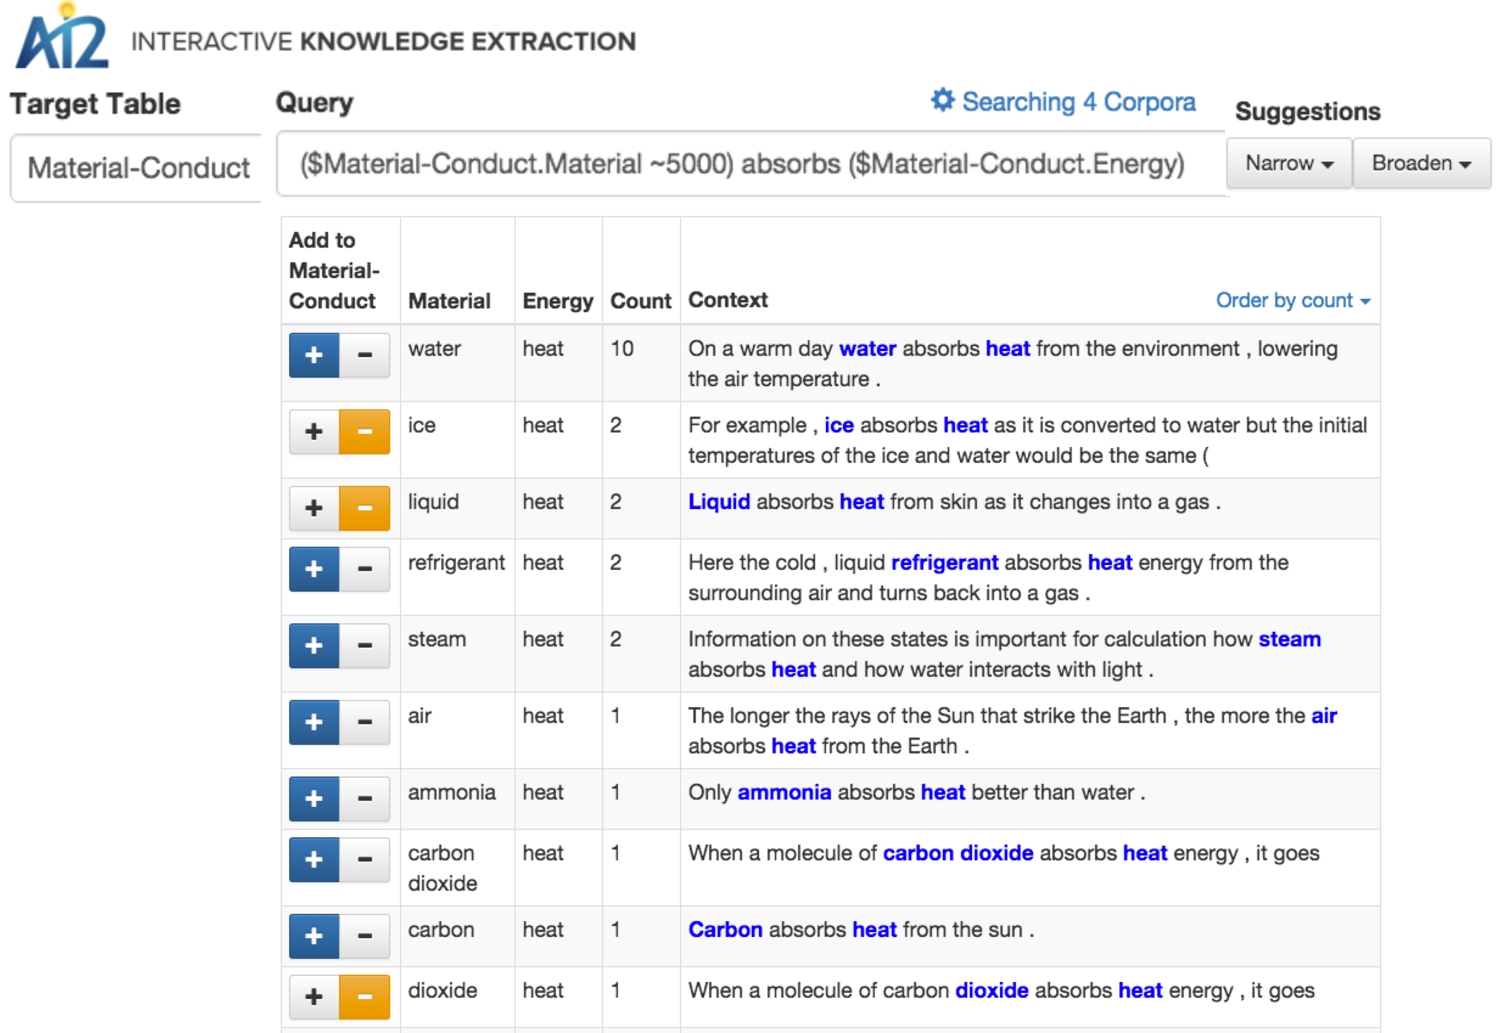
\includegraphics[width=1.8\columnwidth]{./figures/IKE_relation_learning_2.pdf}
\caption{Use of set expansion to find and select vector-similar phrases in the corpus.}
\label{material}
\end{figure*}

\subsection{IKE Query Language}

Central to IKE is the notion that an {\it extraction pattern} can be treated as a {\it search query} over a corpus.
To make this operational, the query language must be both comprehensible and fast to execute.
To meet these requirements, IKE indexes and searches the corpus using a chunk-based rather than parse-based 
representation of the text corpus. The query language
supports wildcards, window sizes, POS tags, chunk tags, as well as reference to other predicate tables already constructed.
In particular, ``capture groups'', indicated by parentheses,
instruct IKE to catch the matching element(s) as candidate entries in the table being populated.
The query language is presented by example in Table\ref{table:query-language}.

\begin{table}[bth]
\noindent\hspace{-0.3cm}
\begin{tabular}{|p{2.2cm}p{5.3cm}|} \hline
\underline{Query} & \underline{Interpretation} \\
{\bf the dog} & matches ``the'' followed by ``dog'' \\
{\bf "brown dog"} & matches the phrase ``brown dog'' \\
{\bf NP grows} & an NP followed by ``grows'' \\
{\bf (NP) grows} & {Capture NP as an entry in the table's column 1} \\
\multicolumn{2}{|l|}{\bf (NP) conducts (NP)} \\
& {Capture both NPs as arg1, arg2} \\
\multicolumn{2}{|l|}{\bf (?$<$myGroup$>$ NP) grows} \\
& {Name the capture group ``myGroup''} \\
{\bf the \{cat,dog\}} & {``the'' followed by ``cat'' or ``dog''}\\
\multicolumn{2}{|l|}{\bf cats and \{NN,NNS\}} \\
& {``cats and'' followed by NN or NNS} \\
{\bf JJ* dog} & Zero or more JJ then ``dog'' \\
{\bf JJ+ dog} & One or more JJ then ``dog'' \\
{\bf JJ[2-4] dog} & 2 to 4 JJ then ``dog'' \\
{\bf dog$~$50} & {Matches ``dog'' and the 50 words most distributionally similar to ``dog''}\\
{\bf . dog} & Any word then ``dog'' \\
{\bf \$colors} & {Any entry in the single-column ``colors'' table}\\
{\bf \$colors$~$100} & {same plus 100 most similar words} \\
{\bf \$flower.color} & {Any in the ``color'' column of ``flower'' table} \\ \hline
\end{tabular}
\caption{IKE's Query Language}
\label{table:query-language}
\end{table}

\subsection{Example Workflow} \label{sect:IKE-workflow}

\begin{figure}[bth]
\begin{center}
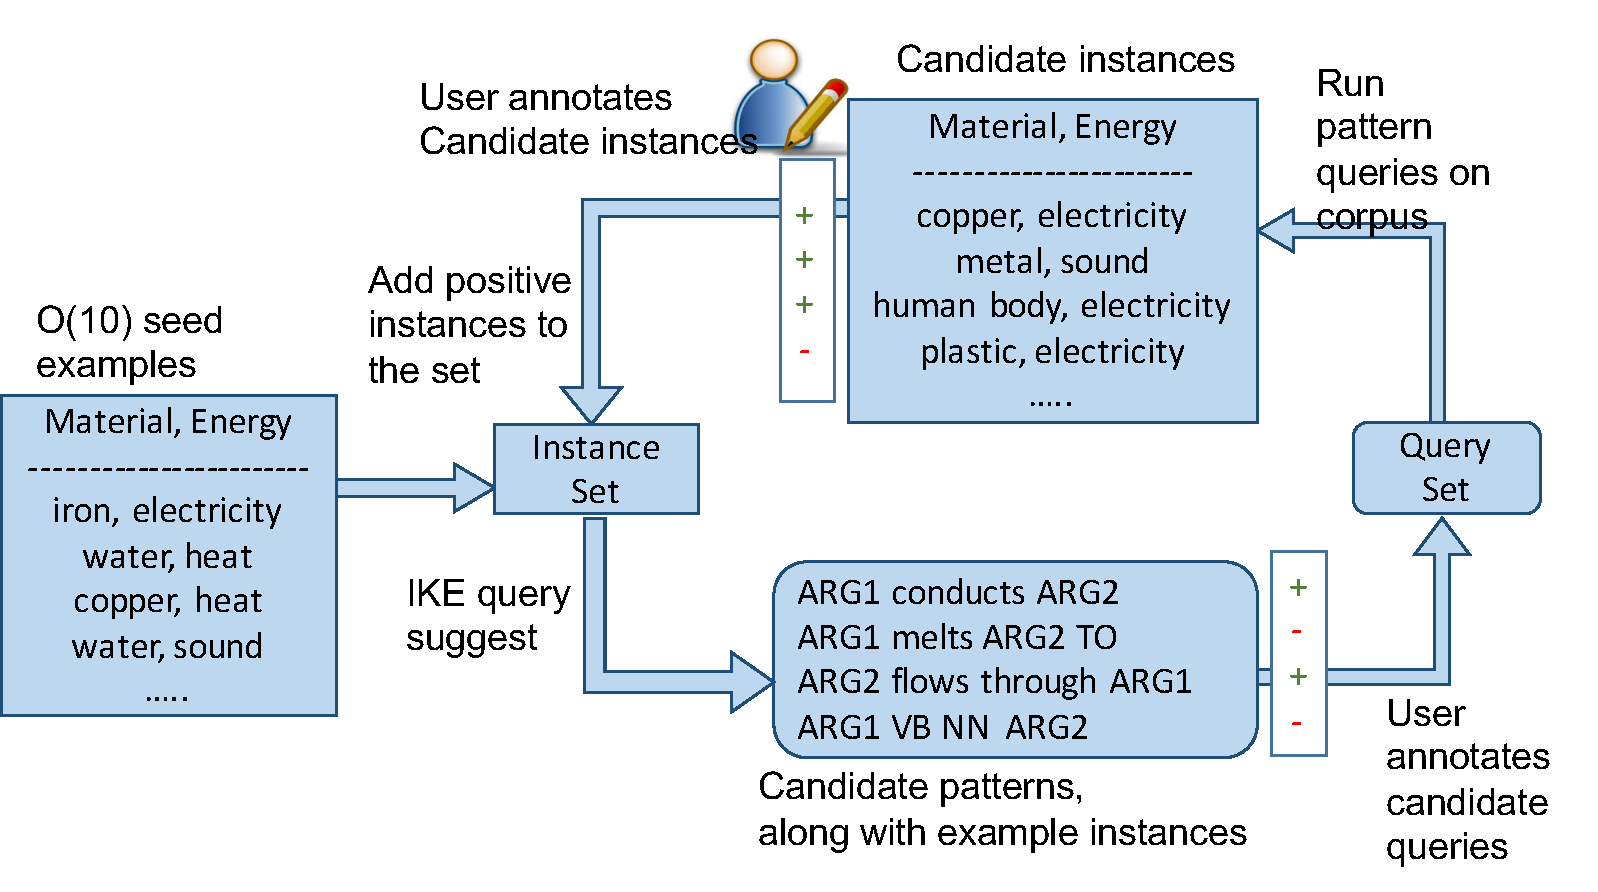
\includegraphics[width=\columnwidth] {./figures/IKE_bootstrapping_ME_3.pdf}
\caption{IKE interactive bootstrapping work-flow to create Material-Conductivity table}
\label{fig:IKE-Bootstrapping}
\end{center}
\end{figure}

We now describe these features in more detail by way of an example. Consider the task of acquiring instances of the binary predicate {\pred conducts}({\it material},{\it energy}), e.g., conducts(``steel'',``electricity''). In IKE, relations are visualized as tables, so we treat this task as one of table population. The user's workflow can be summarized as follows:
\begin{enumerate}[noitemsep]
\item Define the types {\it material} and {\it energy}
\item Create a two-column table for {\pred conducts}
\item Use a seed pattern, e.g., {\bf X:{\it material} conducts Y:{\it energy}}, to populate the {\pred conducts} table with pairs (X,Y)
\item Repeat:
\begin{enumerate}[noitemsep]
  \item Use the ML-based query suggestor to find additional patterns relating the Xs and Ys, i.e., also expressing {\pred conducts}.
  \item Use those additional patterns to further populate {\pred conducts}
  \end{enumerate}
\end{enumerate}
This is the typical bootstrapping algorithm, here with a user in the loop. We now describe each of these steps.

\subsubsection{Define the types {\it material} and {\it energy}}

To define a type, IKE lets a user build a single column table. For example, for type {\it material}, the user:
\begin{enumerate}[noitemsep]
\item Creates a single column table called Material.
\item Manually adds several representative examples in the table, e.g., ``iron'', ``wood'', ``steel''.
\item Expands this set by searching for cosine-vector-similar phrases in the corpus, and marking valid and invalid members (Figure~\ref{material}). The syntax {\bf \$material $\sim$20} denotes the 20 phrases most similar to any existing member in the {\it material} table, where similar is defined as the cosine vector between the phrase embeddings.
The parentheses ``()'' tells IKE that each result is a candidate new member for this table.
\item Repeat step 3 until the table adequately characterizes the intended notion of {\it material}
\end{enumerate}
The process is repeated for the type Energy.

\subsubsection{Create and Seed the {\pred conducts} Table}

The user next creates a two-column table {\pred conducts}, and then uses a seed pattern to find initial pairs to populate it, e.g., the pattern
\begin{quote}
{\bf (\$Material) conducts (\$Energy)}
\end{quote}
extracts pairs of materials and energies they conduct. The user selects valid pairs to initially populate the table. Invalid pairs (negative examples) are also recorded by IKE.

\subsubsection{Bootstrapping to Expand the Table}

%\begin{figure}
%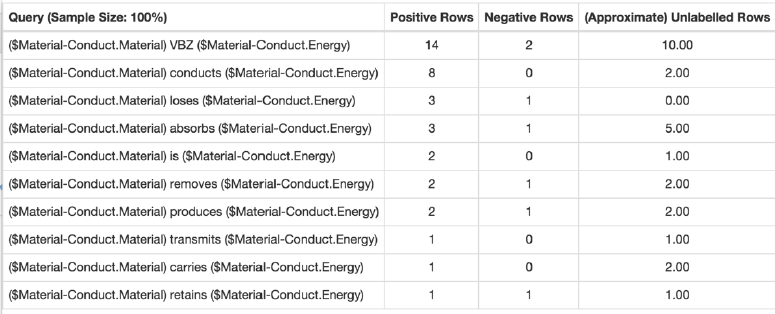
\includegraphics[width=\columnwidth]{./figures/query-suggestor.png}
%\caption{IKE's Query Suggestor proposes additional patterns for the {\pred conducts} relation.}
%\label{query-suggestor}
%\end{figure}

The user can now bootstrap by invoking the Query Suggestor to find additional patterns (queries) that express the target relation.
% , illustrated in Figure~\ref{query-suggestor}. 
It does so by searching for narrowings or broadenings of the current query that cover a large number of positive pairs and a few negative pairs in the table so far. The user then clicks on one of these patterns to select and execute it (possibly with edits if desired) to find more instances of the relation, marks good/bad pairs, and expands the table. This process can then be repeated.

Narrowing involves searching the space of restrictions on the current query, e.g., replacing a POS tag with a specific word, whereas the broaden feature generalizes the given user query e.g. replacing a word by its POS tag. In both cases the candidate queries are ranked based on the number of positive, negative, and unlabeled instances it produces. 
% Figure \ref{query-suggestor} shows an example of narrowing a query for the {\pred conducts} table, where IKE has suggested several verbs found in the corpus, ranked by their ability to distinguish known positives from negatives in the table.
Although the suggested queries can sometimes look complicated with POS and chunk tags within them, the user only has to understand them, not author them from scratch. Hence the required skill set and data analysis workload on the user is significantly reduced. The system still gives control to the user by letting him/her filter/edit the queries, and annotate the extractions in each iteration. 

By repeating this process, the user rapidly populates the table with positive examples. Negative examples are also recorded by IKE for use by the Query Suggestor.

\subsection{Execution Speed}

IKE uses BlackLab \cite{blacklab-tool} for indexing the corpus. This, combined with the chunk-based representation, results in very fast query execution times
(e.g., $<$1 second for a query over 10M sentences), an essential requirement for an interactive system (Table~\ref{table:query-times}).

\begin{table}[tbh]
\centering
\boldmath
\scalebox{0.75}{%
 \begin{tabular}{|l|c|c|} \hline
Corpus & \# sentences & Avg. query-time (sec.) \\
\hline
Barrons & 1.2K & 0.2533	\\ 
CK12 & 17K   & 0.2862	\\ 
SimpleWikipedia & 1M & 0.5296	\\
Web Subset (small) & 1.5M & 0.5953	\\ 
Web Subset (large) & 20M & 2.809 \\
\hline
\end{tabular}
}
\caption{Avg. query-times with different sized corpora.}
\label{table:query-times}
\end{table}

\section{Experimental Evaluation} \label{sect:expt-eval}

\subsection{Experiments}

Although IKE is still under development, we have conducted a small, preliminary evaluation, comparing it with two other methods for populating relation tables. Our interest is in how these different methods compare in terms of precision, yield and time. The methods compared were:
\squishlist
\item \emph{Manual}: The user manually authors and refines patterns (without any automatic assistance) to populate a table.
\item \emph{Automatic}: The user provides an initial table with a few entries, and then lets the system bootstrap on its own, without any further interaction.
\item \emph{Interactive (IKE)}: Interactive bootstrapping, as described earlier.
\squishend
The manual system was implemented in IKE by disabling the embedding-based set expansion and query suggestion features. The automatic approach was simulated in IKE by removing both user annotation steps in Figure \ref{sect:IKE-workflow}, and instead adding all patterns and instances that occur at least $k$ times in the corpus (using $k$ = 2).

\subsection{Tasks and Datasets}

We compared these methods to define and populate two target relations: {\pred has-part}({\it animal},{\it bodypart}), and {\pred conducts}({\it material},{\it energy}).
% {\pred pollution}({\it source}, {\it pollutant}).
All methods extract knowledge from the same corpora of science text, consisting of $\sim$1.5M sentences (largely) about elementary science drawn from science textbooks, Simple Wikipedia, and the Web. For each relation, two (different) users familiar with IKE were asked to construct these tables. Although this study is small and preliminary, it provides some helpful indicators about the IKE's usefulness.

% make use of following four science text corpora (\#sentences in the parenthesis): Barron's study-guide for 4th grade science (1.2K), CK-12 corpora (17K), Simple Wikipedia ($\sim$1M), and Science subset of Waterloo corpus ($\sim$1.5M) \cite{waterloo-corpus}.

\subsection{Results}

\begin{table}[tbh]
\centering
\boldmath
\scalebox{0.75}{%
 \begin{tabular}{|l|cc|cc|c|} \hline
Method & \multicolumn{2}{|c|}{Acquired Patterns} & \multicolumn{2}{|c|}{Extractions} & Time \\
\cline{2-5}
 & No. of & Average & Number & Yield & in min.\\
 & patterns & Precision & (total) & (+ves) & \\ \hline
\emph{Manual}           &   5 & 66.7 &  24 & 16  & 30 \\
\emph{Automatic}        & 108 & 34.4 & 183 & 63 & -  \\ % \hdashline
\emph{IKE} &  41 & 59.2 & 142 & {\bf 84} & 20 \\ \hline
\end{tabular}
}
\caption{{\pred conducts}({\it material},{\it energy}) table: IKE helps the user discover substantially more patterns than the manual method (41 vs. 5), with similar precision and in less time, resulting in the overall highest yield. Fully automatic bootstrapping produced a large number of low precision patterns and overall lower yield than IKE.} 
\label{table:conducts}
\end{table}

\begin{table}[tbh]
\centering
\boldmath
\scalebox{0.75}{%
 \begin{tabular}{|l|cc|cc|c|} \hline
Method & \multicolumn{2}{|c|}{Acquired Patterns} & \multicolumn{2}{|c|}{Extractions} & Time \\
 \cline{2-5}
 & No. of & Average & Number & Yield & in min. \\
 & patterns & Precision & (total) & (+ves) & \\ \hline
\emph{Manual}           & 11 & 21.0 &  291 & 61 & 40 \\
\emph{Automatic}        & 228 & 3.4 & 1386 & 48 & - \\ % \hdashline
\emph{IKE} 		& 21 & 57.4 & 249  & {\bf 143} &  30 \\ \hline
\end{tabular}
}
\caption{{\pred has-part}({\it organism},{\it bodypart}) table: Again, IKE produces the highest yield by helping the user discover substantially more (21) high-precision (57.4\%) patterns.}
\label{table:body-parts}
\end{table}

%\begin{table*}[tbh]
%\centering
%\boldmath
%\scalebox{0.75}{%
% \begin{tabular}{|l|cc|cc|cc|} \hline
%Method & \multicolumn{2}{|c|}{Acquired Patterns} & \multicolumn{2}{|c|}{Extractions} & \multicolumn{2}{|c|}{Time} \\
% \cline{2-5}
% & No. of & Average & Number & Yield & User time &Avg. query time\\
% & patterns & Precision & (total) & (+ves) & in min. & in sec. (\#queries)\\ \hline
%\emph{Manual}           & 11 & 21.0 &  291 & 61 & 40 & 1.23 (35) \\
%\emph{Automatic}        & 228 & 3.4 & 1386 & 48 & - & 2.6 (25) \\ % \hdashline
%\emph{IKE} & 21 & 57.4 & 249  & {\bf 143} &  30 & 3.17 (24) \\ \hline
%\end{tabular}
%}
%\caption{{\pred has-part}({\it organism},{\it bodypart}) table: Again, IKE produces the highest yield by helping the user discover substantially more (21) high-precision (57.4\%) patterns.}
%\label{table:body-parts}
%\end{table*}

Table \ref{table:conducts} shows the results for building the {\pred conducts}({\it material},{\it energy})table. Most importantly, with IKE the user was able to discover substantially more patterns (41 vs. 5) with similar accuracy (59.2\% vs. 66.7\%) than the manual approach, resulting in a larger table (84 vs. 16 rows) in less time (20 vs. 30 mins). It also shows that fully automatic bootstrapping produced a large number of low quality (34.4\% precision) rules, with an overall lower yield (63 rows). 
Table~\ref{table:body-parts} shows similar results for constructing the {\pred has-part}({\it organism},{\it bodypart}) table, again IKE having the highest overall yield.
Although this is a small study, it suggests that IKE has value for rapid knowledge base construction.

% **** \textbf{an example of n-ary relation with general phrases (Animal, Adaptation, Challenge), where adaptation is ``ADJ BODYPART''}

%-------------------------------------------------------

\subsection{Future Development}

IKE is still under development, with several areas needing further investigation. ...  {\bf elaborate}

% Currently IKE is trying to learn best extraction patterns for a target relation using manual annotations of instances and patterns. There is a possibility of improvement in the sense that the query suggestions for a relation can be based on a model for both arguments along with context between and around them. 
%-------------------------------------------------------
%\newpage
%\clearpage

% \section{Conclusions}  \label{sect:conclusions}

\section{Conclusion}

We have presented IKE, a tool that performs fast, interactive bootstrapping to develop high quality extraction patterns for targeted relations. It is an example of a Machine Teaching approach to knowledge base construction, where the focus is on leveraging the user to rapidly guide the system to good results. The preliminary evaluation comparing with manual and automated approaches, although small, is encouraging as it suggests that IKE makes the best of worlds by improving recall compared with a manual process while retaining precision within acceptable bounds. We are currently using IKE to expand the collection of tables used by the Aristo system \cite{clark:2016}.

%-----------------------------

\subsubsection*{Acknowledgments:} 
We thank Tony Fader, Dirk Groeneveld, Oren Etzioni, and Chris Clark for their critical contributions to IKE.

%\clearpage
%\newpage
\bibliography{references}
\bibliographystyle{abbrv}

\end{document}
